\chapter{System Analysis and Design}
\label{chap:overview}

\section{Requirements Engineering}

System requirements were elicited from university capstone project supervision workflows and structured according to IEEE Std 29148-2018~\cite{ieee29148} for functional specifications and ISO/IEC 25010:2023~\cite{iso25010} for software product quality attributes.

\subsection{Functional Requirements}

Every functional requirement is specified as an atomic, testable obligation assigned to an explicit actor and priority level (\textbf{Must} or \textbf{Should}). Table~\ref{tab:func-reqs} lists the sixteen core functional requirements grouped across five functional subsystems.

{\setlength{\tabcolsep}{3.5pt}
\begin{longtable}{|C{0.10}|L{0.15}|L{0.39}|C{0.11}|L{0.25}|}
\caption{Atomic functional requirements organized by subsystem (IEEE 29148).}\label{tab:func-reqs}\\
\hline
\textbf{ID} & \textbf{Actor} & \textbf{Requirement Specification} & \textbf{Prio.} & \textbf{Acceptance Criterion} \\
\hline
\endfirsthead
\multicolumn{5}{c}{\itshape Table \thetable\ (continued from previous page)}\\
\hline
\textbf{ID} & \textbf{Actor} & \textbf{Requirement Specification} & \textbf{Prio.} & \textbf{Acceptance Criterion} \\
\hline
\endhead
\hline
\multicolumn{5}{r}{\itshape Continued on next page}\\
\endfoot
\hline
\endlastfoot
\multicolumn{5}{|l|}{\textbf{Subsystem 1: Identity, Session Management, and Access Control}} \\
\hline
\textbf{\texttt{FR-01}} & Guest / Student & The system shall register accounts, verify one-time email activation and password-reset tokens, and authenticate sessions via local credentials or Google OAuth2. & \textbf{Must} & Invalid/expired token rejected; revoked JWT returns \textbf{HTTP 401}. \\
\hline
\textbf{\texttt{FR-02}} & All Roles & The system shall enforce Role-Based Access Control (\texttt{user}, \texttt{teacher}, \texttt{admin}), personal API keys, and cross-user ownership checks on every resource. & \textbf{Must} & Cross-user essay/verdict access returns \textbf{HTTP 403} (zero IDOR). \\
\hline
\multicolumn{5}{|l|}{\textbf{Subsystem 2: Document Ingestion, Parsing, and Bidirectional Linking}} \\
\hline
\textbf{\texttt{FR-03}} & Student / Teacher & The system shall accept single and batch manuscript uploads in PDF, DOCX, BibTeX, and RIS formats after validating magic bytes, file size, page count, and monthly quota. & \textbf{Must} & Disguised non-PDF/DOCX or over-quota upload rejected cleanly. \\
\hline
\textbf{\texttt{FR-04}} & Student / Teacher & The system shall stream real-time progress across eight pipeline stages and refund upload quota automatically if an asynchronous job fails permanently. & \textbf{Must} & SSE emits steps 0--7; crashed job refunds quota atomically. \\
\hline
\textbf{\texttt{FR-05}} & Pipeline & The system shall segment uploaded manuscripts into body text, in-text markers with surrounding context, and bibliography entries across 12 citation styles (including Vietnamese laws). & \textbf{Must} & \textbf{$\ge 97\%$} bibliography detection on 310-PDF multi-style suite. \\
\hline
\textbf{\texttt{FR-06}} & Pipeline & The system shall detect scanned or legacy-encoded Vietnamese PDFs and invoke selective Optical Character Recognition (OCR) or encoding normalization. & Should & Scanned pages recorded in document diagnostics metadata. \\
\hline
\textbf{\texttt{FR-07}} & Pipeline & The system shall link every in-text citation marker to its target bibliography entry and classify each edge into one of eight structural mapping statuses. & \textbf{Must} & Orphans, uncited refs, and year mismatches isolated accurately. \\
\hline
\multicolumn{5}{|l|}{\textbf{Subsystem 3: Federated Retrieval and Identifier Validation}} \\
\hline
\textbf{\texttt{FR-08}} & Pipeline & The system shall query the offline scholarly corpus and live registries by domain, recording per-source success, failure, and rate-limit provenance. & \textbf{Must} & Offline recall \textbf{$\ge 99\%$}; \textbf{HTTP 429} distinguished from 0 hits. \\
\hline
\textbf{\texttt{FR-09}} & Pipeline & The system shall validate cited URLs and DOIs against SSRF-safe HTTP probes, Retraction Watch metadata, and Internet Archive snapshots. & \textbf{Must} & Private IP targets blocked; retracted works flagged \textbf{$100\%$}. \\
\hline
\multicolumn{5}{|l|}{\textbf{Subsystem 4: Neuro-Symbolic Verification, Scoring, and Remediation}} \\
\hline
\textbf{\texttt{FR-10}} & Pipeline & The system shall compute lexical, semantic, and cross-lingual (\texttt{VI}$\leftrightarrow$\texttt{EN}) alignment between in-text claims and retrieved source titles/abstracts. & \textbf{Must} & Contradicted claims and cross-lingual matches scored in $[0,1]$. \\
\hline
\textbf{\texttt{FR-11}} & Pipeline & The system shall assign one of five verdict labels, a Platt-calibrated probability, and an ordered list of triggered symbolic rule IDs to each reference. & \textbf{Must} & Test accuracy \textbf{$\ge 98.5\%$}, \textbf{$\text{ECE} \le 0.05$}, \textbf{$100\%$} rule trace. \\
\hline
\textbf{\texttt{FR-12}} & Pipeline & The system shall calculate the five-component Citation Integrity Score (CIS) in $[0, 100]$ and generate bilingual (\texttt{EN}/\texttt{VI}) explanations. & \textbf{Must} & Component weights sum to $1.00$; explanations render in EN \& VI. \\
\hline
\textbf{\texttt{FR-13}} & Student / Teacher & The system shall export sanitized reports (PDF, DOCX, CSV, JSON) and generate repaired bibliographies in APA, IEEE, TDTU, BibTeX, RIS, and DOCX formats. & Should & Repaired entries reflect canonical registry metadata without macros. \\
\hline
\textbf{\texttt{FR-14}} & Student / Public & The system shall issue time-limited cryptographic share links with QR verification receipts for read-only third-party inspection. & Should & Expired or tampered share token returns \textbf{HTTP 404/403}. \\
\hline
\multicolumn{5}{|l|}{\textbf{Subsystem 5: Classroom Cohort Supervision and Platform Administration}} \\
\hline
\textbf{\texttt{FR-15}} & Teacher & The system shall allow teachers to manage classes via join codes, inspect cohort analytics and shared hallucinations, and override verdicts when override permission is granted. & \textbf{Must} & Override updates verdict, recalculates CIS, and logs audit entry. \\
\hline
\textbf{\texttt{FR-16}} & Admin & The system shall allow administrators to manage accounts, promo codes, cache state, upstream circuit breakers, and audit logs. & \textbf{Must} & Circuit-breaker reset and cache clear take effect immediately. \\
\hline
\end{longtable}
}

\subsection{Non-Functional Requirements}

To ensure production readiness on standard university hardware without GPUs, ten quantitative Non-Functional Requirements (NFRs) are mapped to ISO/IEC 25010:2023 quality categories in Table~\ref{tab:nfr-reqs}.

{\setlength{\tabcolsep}{3.5pt}
\begin{longtable}{|C{0.11}|L{0.25}|L{0.40}|L{0.24}|}
\caption{Quantitative non-functional requirements mapped to ISO/IEC 25010:2023.}\label{tab:nfr-reqs}\\
\hline
\textbf{ID} & \textbf{ISO/IEC 25010 Attribute} & \textbf{Quality Requirement} & \textbf{Target Metric / SLA} \\
\hline
\endfirsthead
\multicolumn{4}{c}{\itshape Table \thetable\ (continued from previous page)}\\
\hline
\textbf{ID} & \textbf{ISO/IEC 25010 Attribute} & \textbf{Quality Requirement} & \textbf{Target Metric / SLA} \\
\hline
\endhead
\hline
\multicolumn{4}{r}{\itshape Continued on next page}\\
\endfoot
\hline
\endlastfoot
\textbf{\texttt{NFR-01}} & \textbf{Performance Efficiency} (Time Behaviour) & Warm-cache verification latency for a 50-page capstone report ($\sim$32 references) on CPU hardware. & \textbf{$P_{90} \le 2.5\text{\,s}$} (cold Wide Area Network [WAN] $\le 15\text{\,s}$). \\
\hline
\textbf{\texttt{NFR-02}} & \textbf{Performance Efficiency} (Resource Utilization) & Peak backend Python Resident Set Size (RSS) during a 150-page monograph analysis. & \textbf{$\text{RSS} \le 1.5\text{\,GB}$}; heap $\Delta \le 25\text{\,MB}$. \\
\hline
\textbf{\texttt{NFR-03}} & \textbf{Performance Efficiency} (Capacity) & Simultaneous classroom deadline uploads handled without SQLite lock errors or HTTP 5xx responses. & \textbf{$50$ concurrent uploads, $0\%$ failure}. \\
\hline
\textbf{\texttt{NFR-04}} & \textbf{Reliability} (Fault Tolerance) & Graceful degradation when GROBID or upstream scholarly APIs time out or return HTTP 429. & Automatic PyMuPDF fallback; \textbf{$100\%$ safe abstention} on 429. \\
\hline
\textbf{\texttt{NFR-05}} & \textbf{Functional Suitability} & Zero false hallucination accusations on verified works and well-calibrated confidence probabilities. & False hall.\ \textbf{$\le 0.1\%$}; \textbf{$\text{ECE} \le 0.05$}. \\
\hline
\textbf{\texttt{NFR-06}} & \textbf{Security} (Confidentiality \& Integrity) & Protection against SSRF, IDOR, cross-site scripting, CSV formula injection, and brute-force login. & \textbf{Pinned-IP SSRF block}; salted \texttt{bcrypt} + SHA-256/HMAC tokens. \\
\hline
\textbf{\texttt{NFR-07}} & \textbf{Interaction Capability} (Usability) & Accessible Light and Dark editorial interfaces with progressive disclosure and bilingual localization. & \textbf{WCAG 2.1 AA} ($\ge 4.5:1$ contrast); $0\text{\,px}$ overflow. \\
\hline
\textbf{\texttt{NFR-08}} & \textbf{Performance Efficiency} (Time \& Resource) & Code-split frontend JavaScript delivery for fast initial page rendering over campus networks. & Initial entry chunk \textbf{$\le 250\text{\,kB}$} ($\le 80\text{\,kB}$ gzip). \\
\hline
\textbf{\texttt{NFR-09}} & \textbf{Maintainability} (Modularity \& Testability) & Acyclic 8-layer Python architecture and automated backend, frontend, and browser regression suites. & \textbf{$\ge 2{,}500$} automated tests, $0$ failures. \\
\hline
\textbf{\texttt{NFR-10}} & \textbf{Portability} (Installability \& Replaceability) & Reproducible containerized deployment across Linux and macOS CPU hosts without proprietary GPUs. & 3-container health ready \textbf{$\le 60\text{\,s}$}; $0$ GPU dependencies. \\
\hline
\end{longtable}
}

\section{Actors, Access Control, and Use Case Specifications}

\subsection{Role-Based Access Control and Capability Gate}

\textbf{CITRA} serves three primary human actors (\textbf{Student} [\texttt{user}], \textbf{Teacher} [\texttt{teacher}], and \textbf{Administrator} [\texttt{admin}]) alongside external parsing and scholarly registries, as modeled in the UML 2.5 Use Case diagram in Figure~\ref{fig:roles}. Authorization is enforced by reusable FastAPI dependency guards rather than ad-hoc conditionals inside route handlers.

\begin{figure}[H]
    \centering
    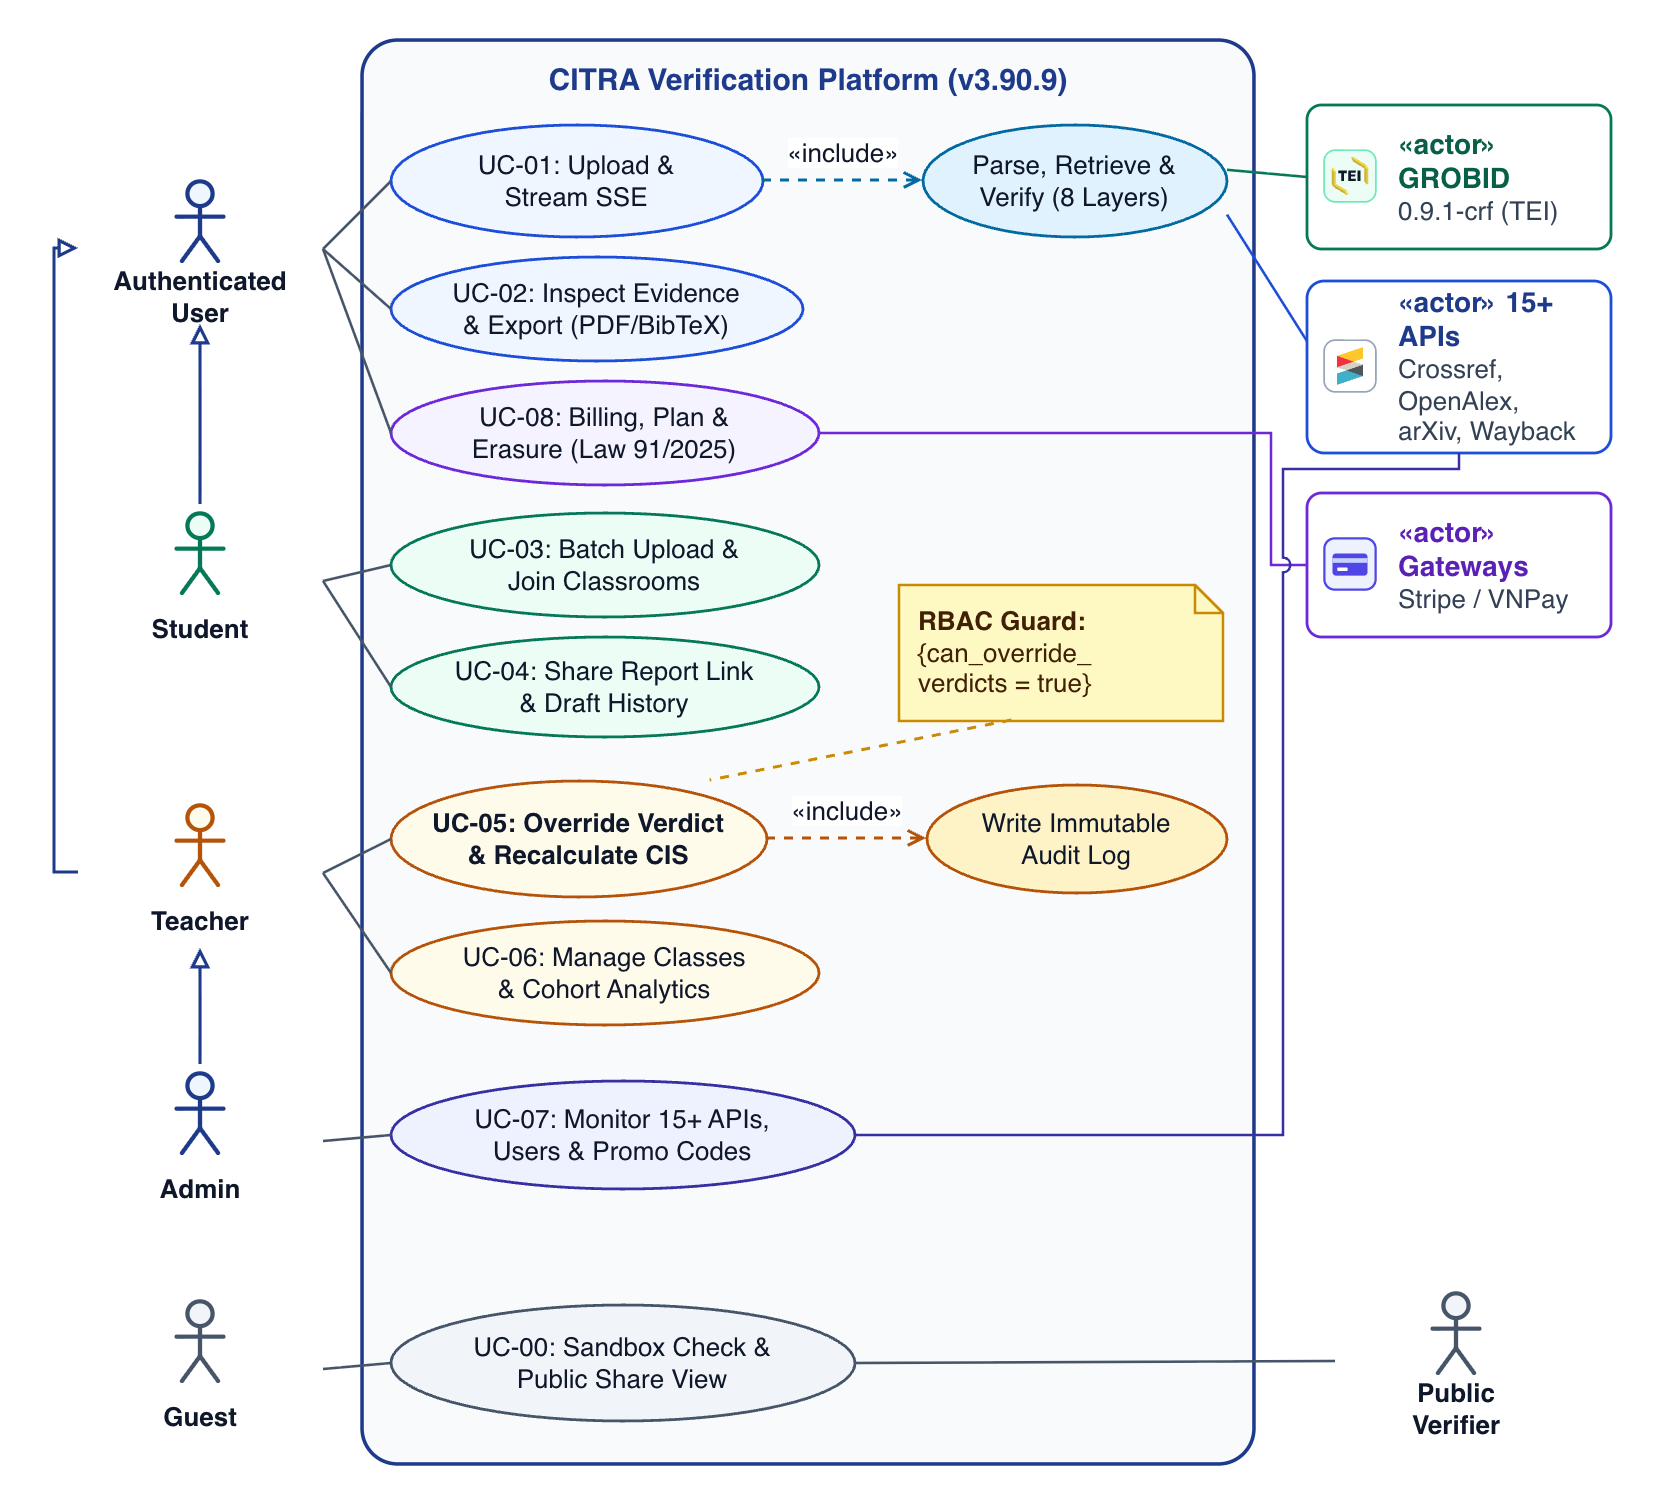
\includegraphics[width=\textwidth,keepaspectratio]{picture/figures/fig3_1_roles.png}
    \caption[UML 2.5 Use Case diagram and RBAC capability gate]{UML 2.5 Use Case diagram across Student, Teacher, and Administrator roles, highlighting the independent \texttt{\{can\_override\_verdicts = true\}} capability guard.}
    \label{fig:roles}
\end{figure}

Crucially, verdict adjudication separates role membership from override authority via an independent boolean column \texttt{users.can\_override\_verdicts}. A faculty member may grant a teaching assistant the \texttt{teacher} role so they can view cohort submissions and triage the pending-review queue, while keeping \texttt{can\_override\_verdicts = False} so only the lead supervisor can reverse a \texttt{suspected\_hallucination} verdict.

\subsection{Core Use Case Specifications}

Table~\ref{tab:uc01}, Table~\ref{tab:uc02}, Table~\ref{tab:uc03}, Table~\ref{tab:uc04}, and Table~\ref{tab:uc05} specify the five primary use cases governing manuscript verification, bibliography repair, instructor adjudication, cohort supervision, and platform administration.

\begin{longtable}{|L{0.24}|L{0.76}|}
\caption{Use Case Specification UC-01: Upload Manuscript and Stream Verification.}\label{tab:uc01}\\
\hline
\textbf{Field} & \textbf{Specification} \\
\hline
\endfirsthead
\multicolumn{2}{c}{\itshape Table \thetable\ (continued from previous page)}\\
\hline
\textbf{Field} & \textbf{Specification} \\
\hline
\endhead
\hline
\multicolumn{2}{r}{\itshape Continued on next page}\\
\endfoot
\hline
\endlastfoot
\textbf{Use Case ID \& Name} & \textbf{UC-01:} Upload Manuscript and Stream Verification (\texttt{FR-03}--\texttt{FR-12}) \\
\hline
\textbf{Primary Actor} & Student (\texttt{user}) or Teacher (\texttt{teacher}) \\
\hline
\textbf{Preconditions} & Actor is authenticated with an active session and remaining monthly upload quota $\ge 1$. \\
\hline
\textbf{Postconditions} & \texttt{essays}, \texttt{citations}, and \texttt{verdicts} rows are persisted; CIS and style profile are stored. \\
\hline
\textbf{Main Success Scenario} & \textbf{1.} Actor selects a \texttt{.pdf}, \texttt{.docx}, \texttt{.bib}, or \texttt{.ris} file (optionally choosing an enrolled class). \newline \textbf{2.} Backend validates magic bytes, size, page limit, and atomically decrements quota via Compare-And-Swap (CAS). \newline \textbf{3.} Backend persists \texttt{EssayRecord(job\_status='queued')} and enqueues the job in \texttt{PipelineAdmissionController}. \newline \textbf{4.} Client subscribes to \texttt{GET /api/essays/\{id\}/events} (SSE) and renders stages 0--7 in real time. \newline \textbf{5.} Worker completes extraction, linking, retrieval, matching, symbolic/ML checking, and CIS scoring, marking \texttt{job\_status='completed'}. \newline \textbf{6.} Client navigates to \texttt{/verification/report/\{id\}}. \\
\hline
\textbf{Alternative / Exception Flows} & \textbf{2a. Invalid MIME or magic bytes:} Backend returns HTTP 400; quota is untouched. \newline \textbf{2b. Quota exhausted:} Backend returns HTTP 402/429; UI displays plan upgrade modal. \newline \textbf{5a. GROBID or external API timeout:} Pipeline switches to PyMuPDF fallback or emits \texttt{R-RATE-LIMITED-ABSTAIN} (\texttt{unresolved}) without failing the job. \newline \textbf{5b. Unrecoverable worker crash:} Stale-job recovery marks \texttt{failed} and refunds 1 quota unit via CAS. \\
\hline
\end{longtable}

\begin{longtable}{|L{0.24}|L{0.76}|}
\caption{Use Case Specification UC-02: Repair Bibliography and Export Manuscript.}\label{tab:uc02}\\
\hline
\textbf{Field} & \textbf{Specification} \\
\hline
\endfirsthead
\multicolumn{2}{c}{\itshape Table \thetable\ (continued from previous page)}\\
\hline
\textbf{Field} & \textbf{Specification} \\
\hline
\endhead
\hline
\multicolumn{2}{r}{\itshape Continued on next page}\\
\endfoot
\hline
\endlastfoot
\textbf{Use Case ID \& Name} & \textbf{UC-02:} Repair Bibliography and Export Manuscript (\texttt{FR-13}) \\
\hline
\textbf{Primary Actor} & Student (\texttt{user}) or Teacher (\texttt{teacher}) \\
\hline
\textbf{Preconditions} & Target essay belongs to Actor (or Actor's supervised class) and \texttt{job\_status='completed'}. \\
\hline
\textbf{Postconditions} & Formatted bibliography strings or repaired \texttt{.docx} / report files are downloaded cleanly. \\
\hline
\textbf{Main Success Scenario} & \textbf{1.} Actor clicks \textit{Fix \& Format Citations} on the report header. \newline \textbf{2.} Backend (\texttt{GET /api/essays/\{id\}/remediate}) maps verified and metadata-erroneous citations to canonical registry fields while isolating \texttt{suspected\_hallucination} entries for manual removal. \newline \textbf{3.} Actor selects target style (\texttt{APA 7th}, \texttt{IEEE}, \texttt{TDTU}, \texttt{BibTeX}, or \texttt{RIS}) and previews field-level diffs. \newline \textbf{4.} Actor downloads the repaired \texttt{.docx} manuscript or sanitized PDF/CSV/JSON audit report. \\
\hline
\textbf{Alternative / Exception Flows} & \textbf{2a. Citation is suspected hallucination:} System refuses to fabricate replacement metadata and marks entry \texttt{hallucination} for author deletion. \\
\hline
\end{longtable}

\begin{longtable}{|L{0.24}|L{0.76}|}
\caption{Use Case Specification UC-03: Adjudicate and Override Citation Verdict.}\label{tab:uc03}\\
\hline
\textbf{Field} & \textbf{Specification} \\
\hline
\endfirsthead
\multicolumn{2}{c}{\itshape Table \thetable\ (continued from previous page)}\\
\hline
\textbf{Field} & \textbf{Specification} \\
\hline
\endhead
\hline
\multicolumn{2}{r}{\itshape Continued on next page}\\
\endfoot
\hline
\endlastfoot
\textbf{Use Case ID \& Name} & \textbf{UC-03:} Adjudicate and Override Citation Verdict (\texttt{FR-15}) \\
\hline
\textbf{Primary Actor} & Teacher (\texttt{teacher}) or Administrator (\texttt{admin}) with \texttt{can\_override\_verdicts = True} \\
\hline
\textbf{Preconditions} & Essay belongs to a class owned by Teacher (or Actor is Admin); target verdict belongs to that essay. \\
\hline
\textbf{Postconditions} & Verdict label updated, essay CIS recomputed, and \texttt{audit\_logs} row inserted in one transaction. \\
\hline
\textbf{Main Success Scenario} & \textbf{1.} Teacher inspects a flagged citation in the Reference Inspector or Pending Reviews queue. \newline \textbf{2.} Teacher selects a new verdict label (e.g.\ \texttt{verified}) and enters a written justification note. \newline \textbf{3.} Backend (\texttt{POST /api/essays/\{id\}/verdicts/\{vid\}/override}) verifies RBAC, capability flag, and essay-to-verdict ownership. \newline \textbf{4.} Within a single DB transaction, backend updates \texttt{VerdictRecord}, re-runs \texttt{CISCalculator.compute()}, updates \texttt{EssayRecord.cis\_json}, and inserts an \texttt{AuditLog} entry. \newline \textbf{5.} UI refreshes the CIS score ring and displays the override badge. \\
\hline
\textbf{Alternative / Exception Flows} & \textbf{3a. Capability flag is False:} Backend aborts with HTTP 403 Forbidden. \newline \textbf{3b. Verdict ID belongs to another essay (IDOR attempt):} Backend aborts with HTTP 404/403. \\
\hline
\end{longtable}

\begin{longtable}{|L{0.24}|L{0.76}|}
\caption{Use Case Specification UC-04: Supervise Classroom Cohort and Shared Anomalies.}\label{tab:uc04}\\
\hline
\textbf{Field} & \textbf{Specification} \\
\hline
\endfirsthead
\multicolumn{2}{c}{\itshape Table \thetable\ (continued from previous page)}\\
\hline
\textbf{Field} & \textbf{Specification} \\
\hline
\endhead
\hline
\multicolumn{2}{r}{\itshape Continued on next page}\\
\endfoot
\hline
\endlastfoot
\textbf{Use Case ID \& Name} & \textbf{UC-04:} Supervise Classroom Cohort and Shared Anomalies (\texttt{FR-15}) \\
\hline
\textbf{Primary Actor} & Teacher (\texttt{teacher}) \\
\hline
\textbf{Preconditions} & Teacher is authenticated and owns at least one classroom cohort. \\
\hline
\textbf{Postconditions} & Cohort analytics, shared hallucination clusters, and ZIP/CSV gradebooks are generated. \\
\hline
\textbf{Main Success Scenario} & \textbf{1.} Teacher creates a class and shares the generated \texttt{join\_code} (default format \texttt{CITRA-XXXX}) with students. \newline \textbf{2.} Students enroll via \texttt{POST /api/teacher/classes/join} and attach project report uploads to the class. \newline \textbf{3.} Teacher opens \texttt{/teacher/classes/\{classId\}}; backend aggregates cohort CIS bands, 5-year citation recency, top triggered rules, and identical fabricated citations appearing across multiple students. \newline \textbf{4.} Teacher exports sanitized CSV summary or bulk ZIP archive of cohort reports. \\
\hline
\textbf{Alternative / Exception Flows} & \textbf{2a. Compromised join code:} Teacher regenerates \texttt{join\_code} without dropping existing members. \\
\hline
\end{longtable}

\begin{longtable}{|L{0.24}|L{0.76}|}
\caption{Use Case Specification UC-05: Monitor System Telemetry and Reset Circuit Breakers.}\label{tab:uc05}\\
\hline
\textbf{Field} & \textbf{Specification} \\
\hline
\endfirsthead
\multicolumn{2}{c}{\itshape Table \thetable\ (continued from previous page)}\\
\hline
\textbf{Field} & \textbf{Specification} \\
\hline
\endhead
\hline
\multicolumn{2}{r}{\itshape Continued on next page}\\
\endfoot
\hline
\endlastfoot
\textbf{Use Case ID \& Name} & \textbf{UC-05:} Monitor System Telemetry and Reset Circuit Breakers (\texttt{FR-16}) \\
\hline
\textbf{Primary Actor} & Administrator (\texttt{admin}) \\
\hline
\textbf{Preconditions} & Actor is authenticated with \texttt{role = 'admin'}. \\
\hline
\textbf{Postconditions} & Upstream provider circuit breakers or expired cache entries are safely reset; telemetry is refreshed. \\
\hline
\textbf{Main Success Scenario} & \textbf{1.} Admin navigates to \texttt{/admin/system}. \newline \textbf{2.} Backend (\texttt{GET /api/system/health}) reports GROBID readiness, SQLite WAL statistics, cache hit rates, verdict distributions, and per-provider circuit-breaker states (\texttt{closed}, \texttt{half\_open}, \texttt{open}). \newline \textbf{3.} After an external API outage resolves, Admin triggers \texttt{POST /api/system/circuit-breakers/reset} to restore live traffic immediately. \\
\hline
\textbf{Alternative / Exception Flows} & \textbf{2a. GROBID container unreachable:} Health monitor marks parser \texttt{degraded (regex fallback)} while keeping uploads operational. \\
\hline
\end{longtable}

\section{End-to-End Processing and Concurrency Design}

\subsection{Eight-Stage Verification Sequence}

Figure~\ref{fig:workflow} presents the UML 2.5 Sequence Diagram for asynchronous manuscript verification and transactional instructor adjudication. Unlike synchronous request-response pipelines that block HTTP workers and time out on 100-page capstone reports, \textbf{CITRA} decouples upload ingestion from background execution across eight tracked pipeline stages: (0) \texttt{parsing}, (1) \texttt{style\_detection}, (2) \texttt{extracting}, (3) \texttt{linking}, (4) \texttt{retrieving}, (5) \texttt{comparing}, (6) \texttt{checking}, and (7) \texttt{scoring}. At each stage boundary, a thread-safe \texttt{ProgressTracker} publishes structured snapshots over Server-Sent Events (SSE) with automatic time-to-live (TTL) eviction once the client disconnects.

\begin{figure}[H]
    \centering
    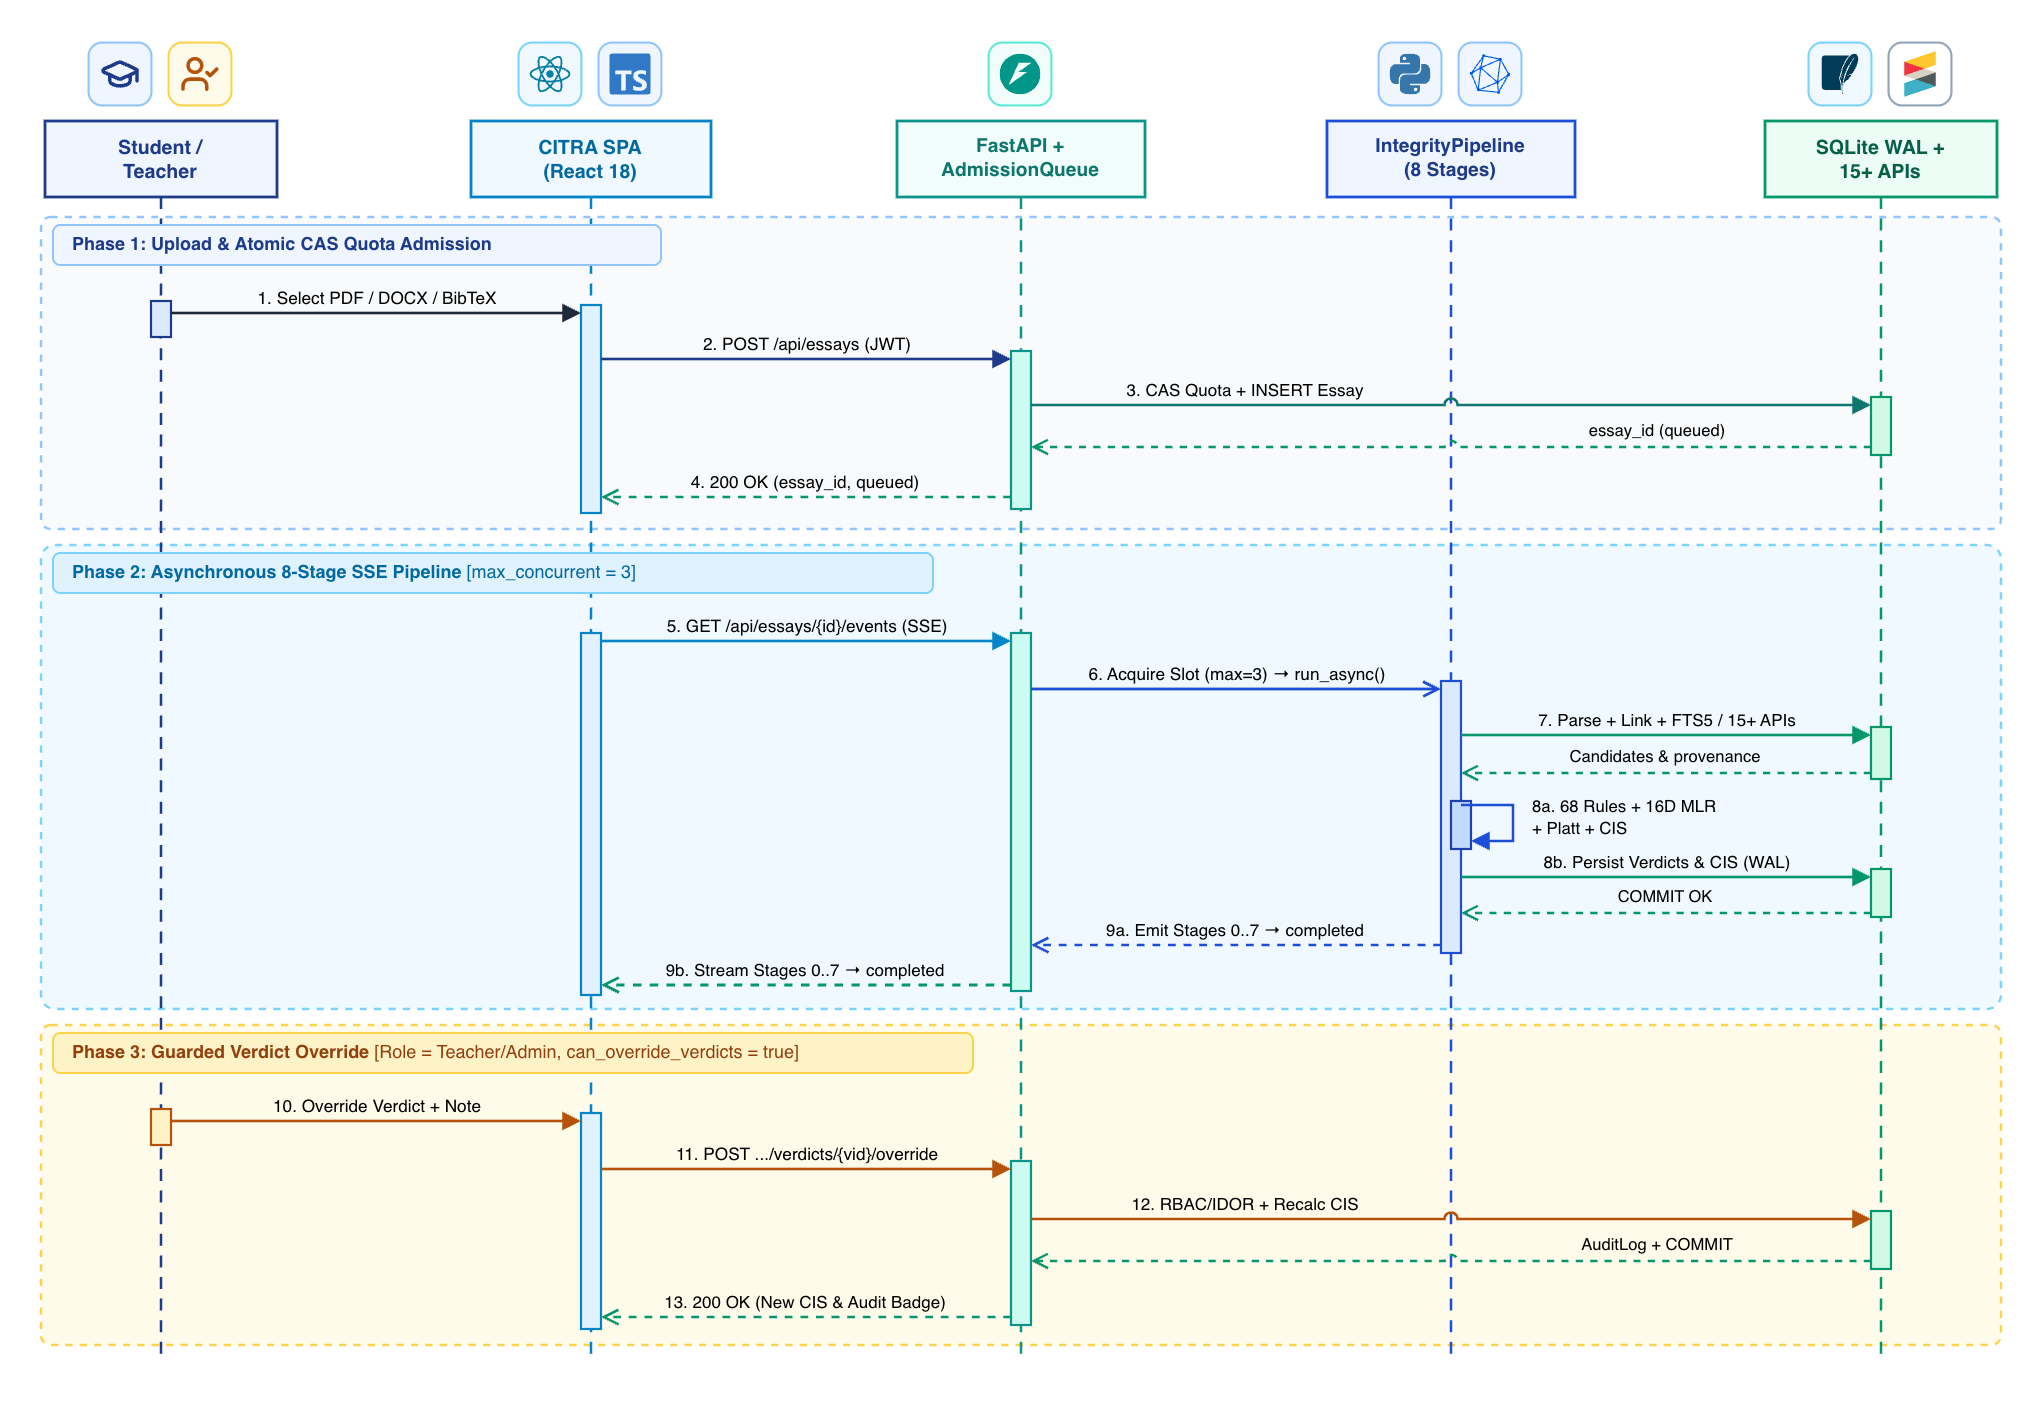
\includegraphics[width=\textwidth,keepaspectratio]{picture/figures/fig3_2_workflow.png}
    \caption[UML 2.5 Sequence diagram for asynchronous verification and teacher override]{UML 2.5 Sequence diagram illustrating asynchronous eight-stage SSE verification and transactional teacher verdict override.}
    \label{fig:workflow}
\end{figure}

\subsection{Admission Control, Worker Modes, and Crash Recovery}

During final submission deadlines, dozens of students may upload project reports simultaneously. Running unbounded Sentence-BERT and GROBID tasks concurrently would exhaust host RAM. \textbf{CITRA} prevents overload through \texttt{PipelineAdmissionController} (\texttt{api/progress.py}), which coordinates slot admission via a thread lock and per-waiter \texttt{asyncio.Event} FIFO queue (\texttt{max\_concurrent = 3} active workers by default) while reporting live \texttt{queue\_position} updates to waiting browsers.

The runtime supports three deployment modes via \texttt{CITRA\_WORKER\_MODE}: \texttt{inline} (single-container FastAPI + background worker), \texttt{web\_only} (API nodes enqueue jobs into SQLite), and \texttt{worker\_only} (dedicated background consumer polling queued jobs with 30-second \texttt{job\_heartbeat\_at} updates). To guarantee crash resilience, \texttt{api/job\_recovery.py} scans for orphaned \texttt{queued} or \texttt{processing} jobs on startup: interrupted jobs below \texttt{MAX\_ORPHAN\_RECOVERY\_ATTEMPTS = 2} are safely re-queued, whereas permanently failed jobs transition to \texttt{failed} and atomically refund the user's monthly upload quota via a Compare-And-Swap (\texttt{quota\_charged: 1 $\rightarrow$ 0}) SQL update so a user is never double-refunded or unfairly billed.

\section{Persistent Data Model and Storage Architecture}

\subsection{Relational Schema and Local FTS5 Corpus}

The persistence layer comprises \textbf{fifteen SQLAlchemy ORM tables} in the primary application database (\texttt{data/app.db}) alongside the read-mostly offline scholarly corpus (\texttt{data/local\_papers.db}, 129,125 records indexed via SQLite FTS5), as summarized in Table~\ref{tab:data-model} and depicted in the Crow's Foot Entity-Relationship Diagram (ERD) in Figure~\ref{fig:data-model}. Public verification share links (\texttt{FR-14}) are issued as stateless HMAC-SHA256 signed tokens (\texttt{sh\_\{eid\}\_\{exp\}\_\{sig\}}) rather than requiring mutable share-session rows.

{\setlength{\tabcolsep}{3.5pt}
\begin{longtable}{|L{0.25}|L{0.46}|L{0.29}|}
\caption{Persistent SQLAlchemy ORM entities in \texttt{db/models.py} (\texttt{v3.90.5}).}\label{tab:data-model}\\
\hline
\textbf{Table Name} & \textbf{Principal Columns and Responsibility} & \textbf{Relationships \& Keys} \\
\hline
\endfirsthead
\multicolumn{3}{c}{\itshape Table \thetable\ (continued from previous page)}\\
\hline
\textbf{Table Name} & \textbf{Principal Columns and Responsibility} & \textbf{Relationships \& Keys} \\
\hline
\endhead
\hline
\multicolumn{3}{r}{\itshape Continued on next page}\\
\endfoot
\hline
\endlastfoot
\textbf{\texttt{users}} & Credentials, OAuth link, \texttt{role}, \texttt{can\_override\_verdicts}, \texttt{plan\_tier}, quota counters, \texttt{created\_at}, \texttt{last\_login\_at} & \textbf{1-to-N} with essays, sessions, tokens, classes, memberships, API keys \\
\hline
\textbf{\texttt{sessions}} & Active bearer \texttt{token} string, \texttt{created\_at}, \texttt{expires\_at} & \textbf{N-to-1} \texttt{users}; revoked on logout or password change \\
\hline
\textbf{\texttt{auth\_tokens}} & One-time SHA-256 \texttt{token\_hash} digests for email activation and password reset & \textbf{N-to-1} \texttt{users}; indexed on \texttt{token\_hash} \\
\hline
\textbf{\texttt{api\_keys}} & \texttt{name}, \texttt{key\_prefix}, SHA-256 \texttt{key\_hash}, \texttt{created\_at}, \texttt{last\_used\_at}, \texttt{is\_active} & \textbf{N-to-1} \texttt{users}; programmatic CLI/API access \\
\hline
\textbf{\texttt{essays}} & \texttt{filename}, \texttt{num\_pages}, \texttt{job\_status}, \texttt{job\_attempt\_count}, \texttt{job\_heartbeat\_at}, \texttt{quota\_charged}, \texttt{style\_profile\_json}, \texttt{cis\_json} & \textbf{N-to-1} \texttt{users} \& optional \texttt{classes}; \textbf{1-to-N} citations, verdicts \\
\hline
\textbf{\texttt{citations}} & Extracted \texttt{in\_text} / \texttt{reference\_list} text, parsed fields, surrounding \texttt{context}, \texttt{mapping\_status}, \texttt{citation\_link\_json} & \textbf{N-to-1} \texttt{essays} (cascade delete) \\
\hline
\textbf{\texttt{verdicts}} & Five-class \texttt{label}, calibrated \texttt{confidence}, \texttt{triggered\_rules}, \texttt{mismatched\_fields}, \texttt{features} JSON, override fields & \textbf{N-to-1} \texttt{essays} (cascade delete); \textbf{1-to-N} \texttt{audit\_logs} \\
\hline
\textbf{\texttt{citation\_cache}} & Normalized query key, serialized multi-source candidate payload, \texttt{hit\_count}, \texttt{created\_at}, \texttt{last\_hit\_at} & Global cross-essay cache reducing redundant API traffic \\
\hline
\textbf{\texttt{classes}} & Cohort name, description, unique \texttt{join\_code} (\texttt{CITRA-XXXX}), \texttt{teacher\_id} & \textbf{N-to-1} \texttt{users} (teacher); \textbf{1-to-N} memberships \& essays \\
\hline
\textbf{\texttt{class\_memberships}} & Student enrollment record linking \texttt{student\_id} to \texttt{class\_id} & \textbf{Unique composite key} \texttt{(class\_id, student\_id)} \\
\hline
\textbf{\texttt{audit\_logs}} & \texttt{verdict\_id}, acting username, \texttt{original\_label}, \texttt{new\_label}, justification \texttt{note}, \texttt{logged\_at} & \textbf{N-to-1} \texttt{verdicts}; no update endpoint \\
\hline
\textbf{\texttt{billing\_transactions}} & Checkout session ID, \texttt{plan\_tier}, \texttt{billing\_cycle}, USD/VND amounts, Stripe / VNPay metadata, \texttt{status} & \textbf{N-to-1} \texttt{users}; payment audit ledger \\
\hline
\textbf{\texttt{promo\_codes}} & Code string, percent/fixed discount, tier/cycle filters, \texttt{max\_uses}, \texttt{used\_count}, \texttt{expires\_at} & \textbf{1-to-N} \texttt{promo\_redemptions} \\
\hline
\textbf{\texttt{promo\_redemptions}} & Applied discount amount, \texttt{promo\_code\_id}, \texttt{user\_id}, \texttt{transaction\_id} & Joins \texttt{promo\_codes}, \texttt{users}, and \texttt{billing\_transactions} \\
\hline
\textbf{\texttt{schema\_migrations}} & Revision \texttt{version} PK (\texttt{0001}--\texttt{0013}), \texttt{name}, SHA-256 \texttt{checksum}, \texttt{execution\_ms}, \texttt{applied\_at} & Startup schema integrity ledger \\
\hline
\end{longtable}
}

\begin{figure}[H]
    \centering
    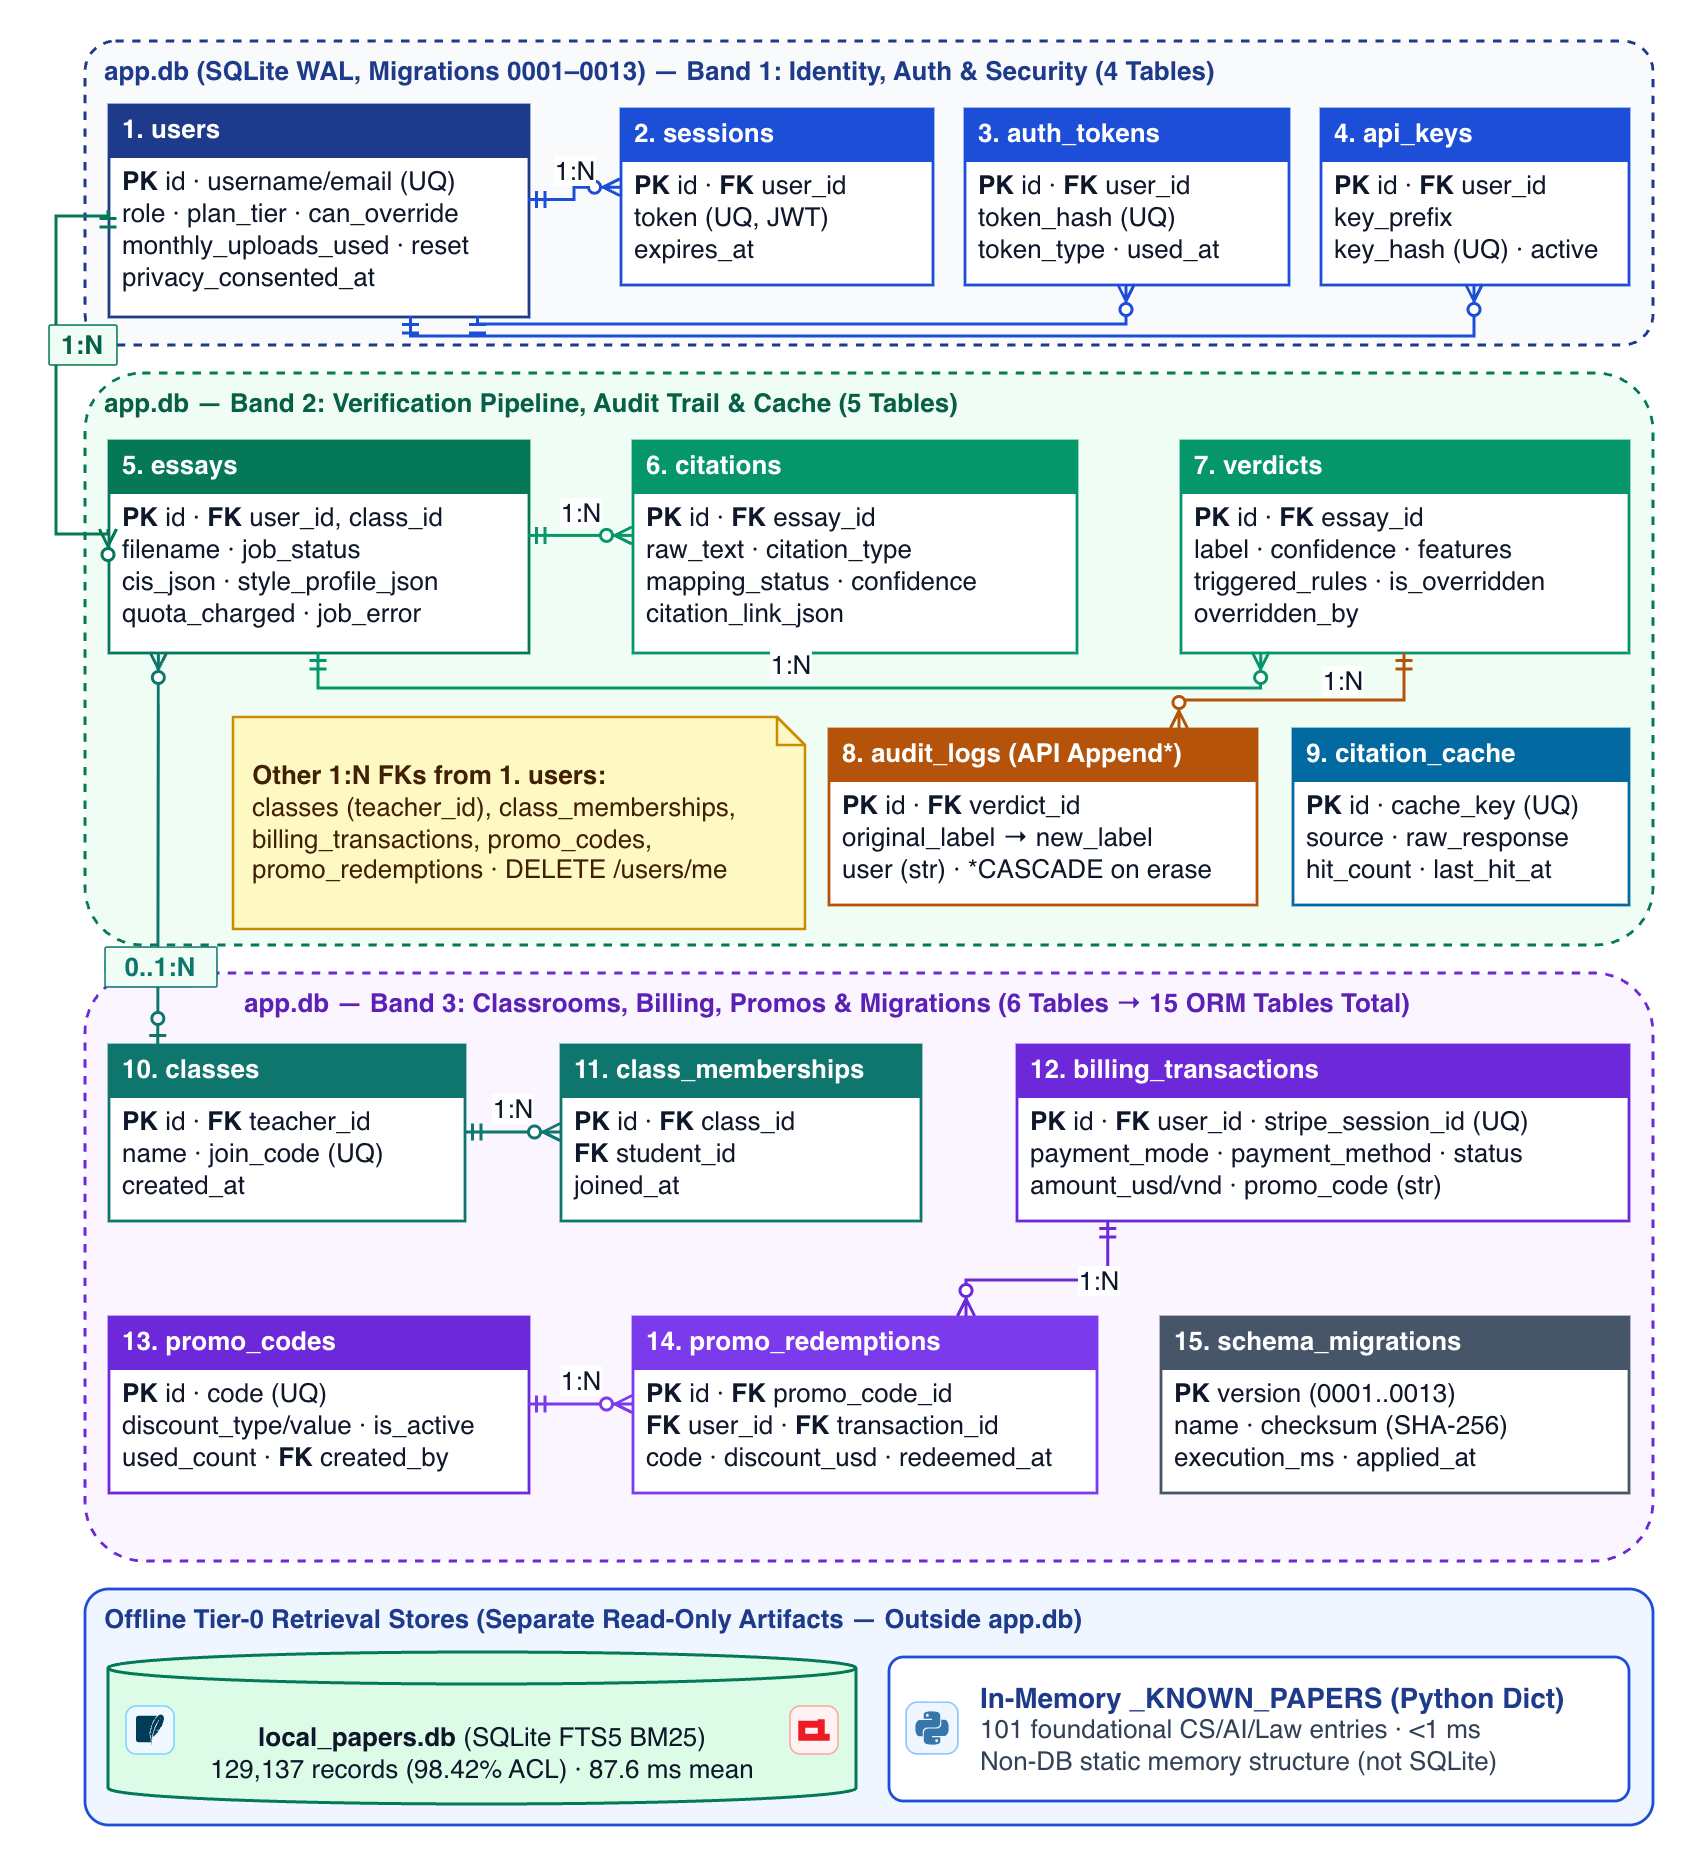
\includegraphics[width=\textwidth,keepaspectratio]{picture/figures/fig3_3_data_model.png}
    \caption[Crow's Foot Entity-Relationship Diagram of the 15-table database schema]{Crow's Foot Entity-Relationship Diagram (ERD) of the 15 application ORM tables (\texttt{app.db}) and the offline 129,125-record SQLite FTS5 scholarly corpus (\texttt{local\_papers.db}).}
    \label{fig:data-model}
\end{figure}

\subsection{Schema Migrations, SQLite WAL Tuning, and Audit Retention}

Schema evolution across versions is managed deterministically by \texttt{db/migrations.py}, which tracks thirteen numbered, SHA-256 checksummed migrations (\texttt{0001}--\texttt{0013}) inside \texttt{schema\_migrations} and verifies checksums at startup to detect accidental schema drift. For concurrent read/write throughput, \texttt{db/sqlite\_tuning.py} configures \texttt{PRAGMA journal\_mode=WAL}, \texttt{synchronous=NORMAL}, and \texttt{busy\_timeout=30000} on native POSIX disks while automatically detecting macOS VirtioFS or network bind mounts (where shared-memory \texttt{-shm} mmap files risk corruption) and switching safely to \texttt{DELETE} journal mode.

Regarding audit retention, \texttt{audit\_logs} exposes no HTTP update or individual delete endpoint during normal operation so that instructor overrides remain tamper-evident. When a user deletes an uploaded essay or executes self-service account deletion (\texttt{DELETE /api/users/me}), cascading cleanup removes child \texttt{citations}, \texttt{verdicts}, and associated \texttt{audit\_logs} rows within a single database transaction so referential integrity is preserved without orphaned records.

\section{API Contract, Deployment, and Security Design}

\subsection{REST and SSE API Surface}

All backend endpoints are mounted under the \texttt{/api} prefix in \texttt{api/\allowbreak main.py}~\cite{fastapi}, as detailed in Table~\ref{tab:api-surface}. Synchronous SQLite and filesystem operations run inside thread-pool executors so the main \texttt{asyncio} loop never blocks active SSE streams.

{\setlength{\tabcolsep}{3.5pt}
\begin{longtable}{|L{0.31}|L{0.69}|}
\caption{FastAPI REST and SSE endpoint groups mounted under \texttt{/api} (\texttt{v3.90.5}).}\label{tab:api-surface}\\
\hline
\textbf{Route Prefix} & \textbf{Principal Endpoints and Operations} \\
\hline
\endfirsthead
\multicolumn{2}{c}{\itshape Table \thetable\ (continued from previous page)}\\
\hline
\textbf{Route Prefix} & \textbf{Principal Endpoints and Operations} \\
\hline
\endhead
\hline
\multicolumn{2}{r}{\itshape Continued on next page}\\
\endfoot
\hline
\endlastfoot
\textbf{\texttt{/api/auth/*}} & \texttt{POST /register}, \texttt{/login}, \texttt{/google} \textbf{(OAuth2)}, \texttt{/logout}, \texttt{/activate}, \texttt{/forgot-password}, \texttt{/reset-password}, \texttt{GET /me}. \\
\hline
\textbf{\texttt{/api/essays/*}} & \texttt{POST /essays} (upload), \texttt{GET /essays}, \texttt{/essays/stats}, \texttt{/essays/\{id\}/status}, \texttt{/essays/\{id\}/events} \textbf{(SSE)}, \texttt{/essays/\{id\}/report} (\texttt{json|csv|pdf|docx}), \texttt{/essays/\{id\}/remediate}, \texttt{/essays/\{id\}/export-healed-docx}, \texttt{/essays/\{id\}/revision-diff}, \texttt{/essays/\{id\}/page-preview/\{p\}}, \texttt{POST /essays/\{id\}/share}, \texttt{GET /essays/shared/\{token\}}, \texttt{/essays/sandbox/*}. \\
\hline
\texttt{/api/essays/\allowbreak\{id\}/\allowbreak verdicts/*} & \texttt{POST /api/essays/\allowbreak\{id\}/\allowbreak verdicts/\allowbreak\{vid\}/override} (capability-gated teacher override + transactional CIS recalculation). \\
\hline
\textbf{\texttt{/api/teacher/*}} & \texttt{GET /dashboard}, \texttt{/classes}, \texttt{POST /classes/join}, \texttt{/classes/\{id\}/regenerate-code}, \texttt{GET /classes/\{id\}/analytics}, \texttt{/classes/\{id\}/pending-reviews}, \texttt{/classes/\{id\}/export.csv}, \texttt{/classes/\{id\}/export.zip}. \\
\hline
\textbf{\texttt{/api/users/*}} & Admin \texttt{/users} management; self-service \texttt{PATCH/DELETE /users/me}, \texttt{/users/me/password}, \texttt{/users/me/avatar}, and \texttt{/users/me/api-keys}. \\
\hline
\textbf{\texttt{/api/billing/*}} & \texttt{GET /plans}, \texttt{/subscription}, \texttt{POST /create-checkout-session}, Stripe \& VNPay \textbf{HMAC-SHA512} verification, \texttt{/cancel}, and admin \texttt{/admin/promos}. \\
\hline
\textbf{\texttt{/api/system/*}}, \textbf{\texttt{/api/audit/*}}, \textbf{\texttt{/api/cache}}, \textbf{\texttt{/api/export/*}} & \texttt{GET /api/health}, \texttt{GET /api/system/health}, \texttt{POST /api/system/circuit-breakers/reset}, \texttt{DELETE /api/cache}, \texttt{GET /api/audit/log}, \texttt{GET /api/export/report} (admin system summary). \\
\hline
\end{longtable}
}

\subsection{Container Deployment Topology and Defense-in-Depth Security}

Figure~\ref{fig:deployment} depicts the UML 2.5 Deployment Topology across development (\texttt{docker-compose.yml}) and hardened production (\texttt{docker-compose.prod.yml}). Three containers communicate over an isolated Docker bridge network: \texttt{essay-\allowbreak check-\allowbreak grobid} runs \texttt{grobid/grobid:0.9.1-crf} (chosen over heavier deep-learning images so structured PDF parsing runs deterministically within a 2--3\,GB JVM heap on CPU-only servers). Meanwhile, \texttt{integrity-api} runs Uvicorn/FastAPI, and \texttt{integrity-web} serves the compiled SPA via Nginx 1.27 with TLS 1.2/1.3, Content-Security-Policy, HTTP Strict-Transport-Security, and unbuffered SSE proxying (\texttt{X-Accel-Buffering: no}). In production, ports \texttt{8000} and \texttt{8070} bind strictly to internal/loopback interfaces rather than the public Internet.

\begin{figure}[H]
    \centering
    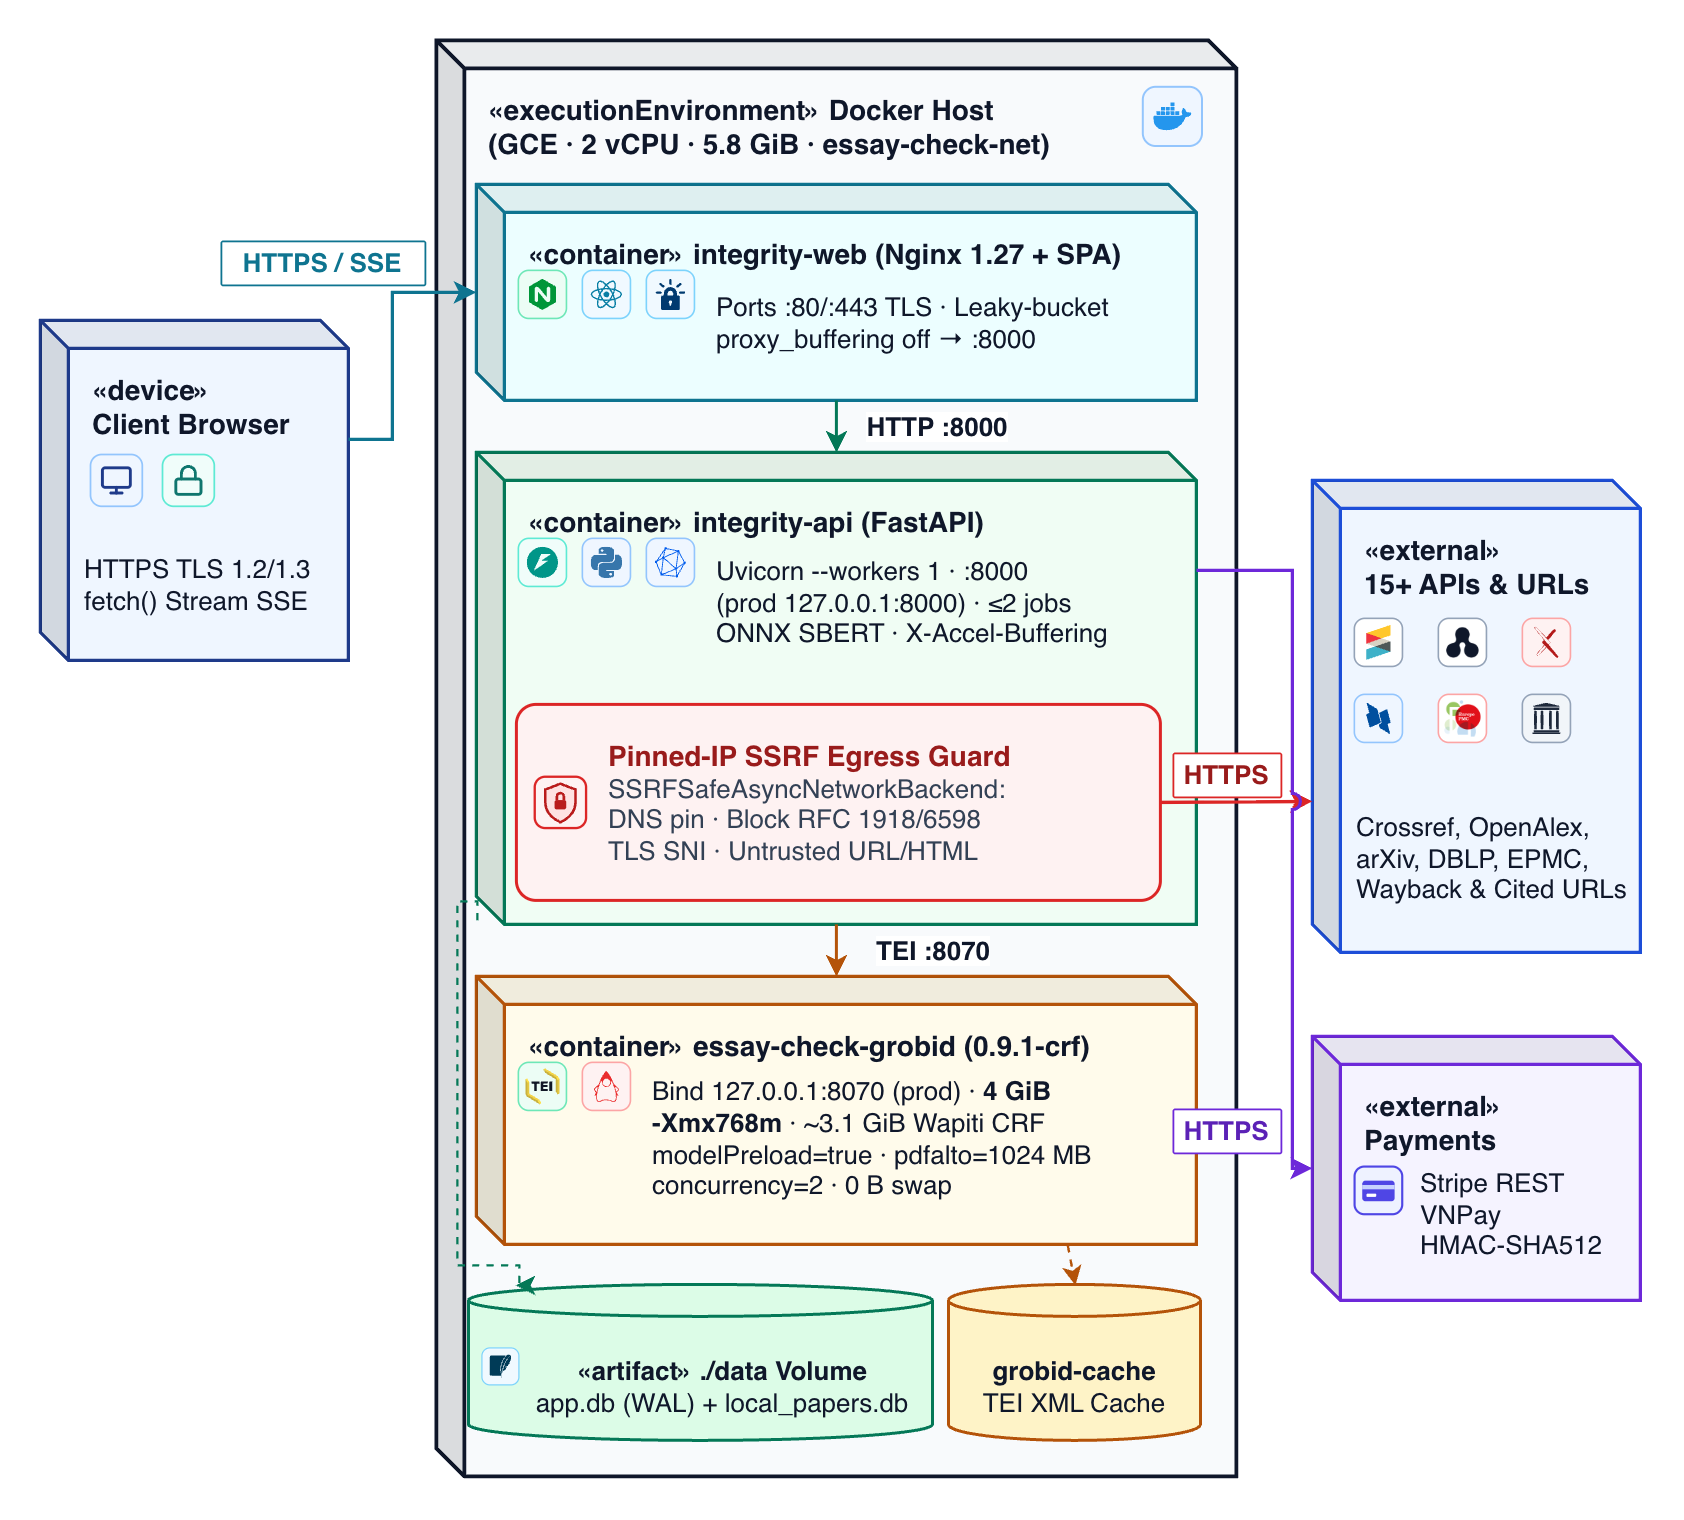
\includegraphics[width=\textwidth,keepaspectratio]{picture/figures/fig3_4_deployment.png}
    \caption[UML 2.5 Deployment diagram of the three-container CITRA platform]{UML 2.5 Deployment topology coordinating Nginx (\texttt{integrity-web}), FastAPI (\texttt{integrity-api}), and CPU-tuned \texttt{grobid:0.9.1-crf} with persistent SQLite volumes.}
    \label{fig:deployment}
\end{figure}

Defense-in-depth security controls span four boundaries:
\begin{itemize}
    \item \textbf{Token and Credential Hardening:} Passwords use salted \texttt{bcrypt} hashes; one-time email tokens (\texttt{auth\_tokens.token\_hash}) and personal API keys (\texttt{api\_keys.key\_hash}) store only SHA-256 digests in SQLite, while public share receipts use stateless HMAC-SHA256 signatures. Production startup aborts if \texttt{JWT\_SECRET} remains at its development placeholder.
    \item \textbf{Pinned-IP SSRF Defense:} The \texttt{LinkValidator} and \texttt{SafeHtml\allowbreak Meta\allowbreak Verifier} modules resolve hostnames prior to connection, block loopback, link-local, RFC 1918 private, and cloud-metadata IP ranges (\texttt{169.254.\allowbreak 169.254}), re-validate every HTTP redirect hop, and connect via a custom \texttt{httpx} transport pinned to the verified IP address to defeat DNS rebinding.
    \item \textbf{Upload and Export Sanitization:} Uploads check PDF (\texttt{\%PDF-}) and ZIP/DOCX (\texttt{PK\textbackslash x03\textbackslash x04}) magic bytes, enforce strict byte/page caps, and neutralize spreadsheet formula prefixes (\texttt{=}, \texttt{+}, \texttt{-}, \texttt{@}) in CSV exports.
    \item \textbf{Anti-IDOR Ownership and Rate-Limiting Guards:} Every essay, verdict, share-token, and classroom endpoint enforces explicit resource-ownership checks (\texttt{user\_id} or supervised \texttt{class\_id}) before returning data, while authentication and upload endpoints enforce token-bucket rate limits and atomic Compare-And-Swap (\texttt{CAS}) quota accounting.
\end{itemize}

\section{Chapter Summary}

This chapter specified sixteen atomic functional requirements (IEEE 29148), ten quantitative non-functional requirements (ISO/IEC 25010), UML 2.5 use case and sequence models, the 15-table SQLAlchemy schema with thirteen SHA-256 checksummed migrations (\texttt{0001}--\texttt{0013}), the \texttt{/api/*} REST/SSE contract, and the security-hardened Docker deployment. Chapter~\ref{chap:architecture} details the internal software architecture and algorithms across all eight pipeline layers.
